\section{Discussion and Outlook}

\begin{figure}[t]
\centering
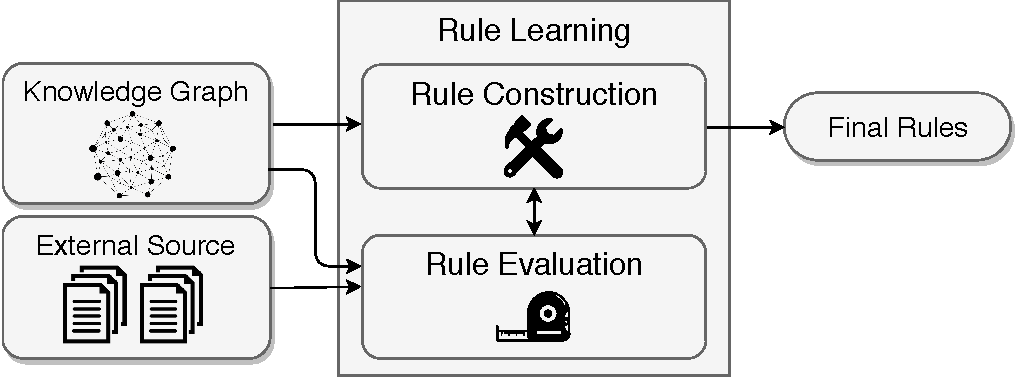
\includegraphics[width=8cm]{figures/discussion_overview}
\caption{Rule learning using external sources.}
\label{fig:discussion_overview}
\end{figure}

In this tutorial, we discussed the different approaches for rule induction and reasoning over real-life KGs. We briefly illustrated the common method for KG construction and the incompleteness and inaccuracy challenges they face. We also illustrated the difference between \textit{Horn} and  \textit{nonmonotonic} logic program and their connection to association rules. Later, we reviewed some of the existing systems for constructing Horn rules from KGs and the proposed rule evaluation measurements under OWA. Furthermore, we discussed the exiting inductive and abductive methods for learning nonmonotonic rules and their applicability over real-life KGs. Finally, we discussed rule revision approach RUMIS, which tries to capture exceptional cases to achieve accurate and consistent predictions. 

Despite the advances in rule learning, the existing methods still learn limited formats for rules, \eg closed rules, with even restrictive language bias. Additionally, they are still prone to KG incompleteness and not being able to determine the possible gaps in the data under OWA. These challenges lead to the generation of uninteresting and noisy rules. Follows some possible directions to overcome such challenges. 


\leanparagraph{Rule Learning with External Sources}  One of the main difference between the existing approaches is the rule evaluation metric which affects the quality of the resulting rule set heavily. However,  existing measures only consider the given KG in their computation, and cover a small subset of the local patterns as well. Other missing facts are not counted, therefore, the estimated quality of rules might be inaccurate.

One promising direction is to consider pieces of evidence from other external resources while estimating the quality of the rules as shown in Figure~\ref{fig:discussion_overview}. This external resource can either be a human expert giving feedback about the correctness of the rule or its predictions similar to~\cite{Dzyuba2017}, a community voting via crowd-sourcing, or a fact-checking over textual resources such as Defacto~\cite{defacto} or FactChecker~\cite{factchecker}. In addition, external KG meta-data could give some information about the existence of certain types of facts within the KG (as in CARL~\cite{carl}).

An alternative relational learning method for KG completion is to learn representations (i.e. embeddings) of entities and relations with the propose of estimating the likelihood of unseen facts. Recently, several models have been proposed, while many of them achieved reasonable results quality~\cite{Wang2017}, yet their predictions are not interpretable~\cite{Shakerin2018}. Furthermore, some of them allow integrating unstructured resources during the training phase. Utilizing such models in the rule learning process can achieve promising results.% as shown in~\cite{thinh_tr}.

\leanparagraph{Learning Other Rule Forms}
Prominent rule learning approaches only extract normal $closed$ logical rules, which may not capture all interesting patterns. However, other rule forms such as rules with disjunction (\eg $isMale(X) \vee isFemale(X) \leftarrow isPerson(X)$) or rules with existential quantifier (\eg $(\exists Y: playsInstrument(X, Y)) \leftarrow isMusician(X))$) can encode more interesting patterns. Even though these rules may not directly infer new facts, they can be used as guidance for the information retrieval approaches.


\leanparagraph{Learning Temporal-aware Rules} Current approaches extract the rules from the directly stated entities and relations. More promising direction would be to learn patterns over more unstated relations such as temporal rules. For examples, KGs usually contains the dates of the events, \eg $\mi{dateOfbirth}$ or $happenedOn$ which are sparse data and requires arithmetic operator to make use of them, \eg $before(X,Y)$, $after(X,Y)$. Learning interesting rules over these data is still not well studied.


\leanparagraph{Learning Hybrid Rules} The number of predicates is limited in most of the KGs. Therefore, sometimes it is hard to learn interesting patterns from the KG only. In contrast, textual resources are rich with verbal phrases that indicate events or relations. However, learning the simplest rules from unstructured resources is challenging. Therefore, it worth investigating constructing hybrid rules that combine both resources.  For example, to learn a rule such as
\vspace{-0.9em}
\begin{align*}
\mi{participatedIn(X,Y)} \leftarrow & \mi{playsFor(X,Z)}, \mi{competes(Z,Y)},\\ & \naf injuredDuring(X,Y)
\end{align*}
The rule encodes that a player participates in a championship if he plays for a competing team unless he was injured during the championship. Learning the positive part of the rule can be easily done over the KG, yet the last one is more common to find in the text. 




%\section{Discussion and Outlook}
%\label{sec:discussion_outlook}
%Toward the rule-based KG completion problem, a number of future directions could be put into consideration.
%\subsubsection{Rule Learning with External Source.}

%In most of rule learning systems have been proposed \cite{amie,op,rdf2rules}, while their rule construction methods may vary, the core of them is at the proposed rule evaluation metric. Various rule measures have been introduced, from the simplest to the most sophisticated one. Nevertheless, most of them are computed based on only the given graph, and cover only a small subset of local patterns in the KG, thus might wrongly estimate the quality of extracted rules since real-world KGs are usually highly incomplete.
%
%One promising possibility to tackle this problem is to incorporate external related data from outside of the KG. The overview of such rule learning system could be described in Figure \ref{fig:discussion_overview}. The KG related external data can be extracted from many sources (e.g. crowd-sourcing, Web-extraction), and is obviously useful not only for rule evaluation, but also for rule construction over the KG. For instance, external data can give some feedback about the quality of predicted facts in several forms such as binary decision (\ie true or false) or a likelihood score. This feedback could be then taken into account for rule quality evaluation or exception capturing. In addition, external KG meta-data could gives some information about the existence of certain types of facts within the KG (as exploited in CARL~\cite{carl}). Moreover, we can also somehow learn rules directly from the text and then apply them back to the KG.
%
%An alternative relational learning method for KG completion is to learn representations (i.e. embeddings) of entities and relations for predicting likelihood of unseen facts. While these methods capture global patterns in the data, the predictions that they produce are not interpretable~\cite{Shakerin2018}. Many such models are been proposed \cite{Wang2017}, in which some of them could even be extended with additional unstructured knowledge (e.g., text corpus). Hence, integrating these embedding models into the rule learning approach might be a potential solution for the problem of rule-based KG completion.
%\subsubsection{Learning Various Rule Forms}
%In the KG completion problem, as mentioned, most of the rule mining approaches only mine $closed$ rules. Nevertheless, other form of rules might be also interesting. For example, rules with disjunction (e.g. $isMale(X) \vee isFemale(X) \leftarrow isPerson(X)$), rules with quantifier (e.g. $(\exists Y: playsInstrument(X, Y)) \leftarrow isMusician(X))$). Even though these kinds of rule do not directly make predictions on the knowledge graph since we do not know exactly which facts of the head are true, they might give us some useful constraints about the knowledge graph.
